\chapter{Stand van zaken}
\label{ch:stand-van-zaken}

% Tip: Begin elk hoofdstuk met een paragraaf inleiding die beschrijft hoe
% dit hoofdstuk past binnen het geheel van de bachelorproef. Geef in het
% bijzonder aan wat de link is met het vorige en volgende hoofdstuk.

% Pas na deze inleidende paragraaf komt de eerste sectiehoofding.
%
%Dit hoofdstuk bevat je literatuurstudie. De inhoud gaat verder op de inleiding, maar zal het onderwerp van de bachelorproef *diepgaand* uitspitten. De bedoeling is dat de lezer na lezing van dit hoofdstuk helemaal op de hoogte is van de huidige stand van zaken (state-of-the-art) in het onderzoeksdomein. Iemand die niet vertrouwd is met het onderwerp, weet er nu voldoende om de rest van het verhaal te kunnen volgen, zonder dat die er nog andere informatie moet over opzoeken \autocite{Pollefliet2011}.
%
%Je verwijst bij elke bewering die je doet, vakterm die je introduceert, enz. naar je bronnen. In \LaTeX{} kan dat met het commando \texttt{$\backslash${textcite\{\}}} of \texttt{$\backslash${autocite\{\}}}. Als argument van het commando geef je de ``sleutel'' van een ``record'' in een bibliografische databank in het Bib\TeX{}-formaat (een tekstbestand). Als je expliciet naar de auteur verwijst in de zin, gebruik je \texttt{$\backslash${}textcite\{\}}.
%Soms wil je de auteur niet expliciet vernoemen, dan gebruik je \texttt{$\backslash${}autocite\{\}}. In de volgende paragraaf een voorbeeld van elk.
%
%\textcite{Knuth1998} schreef een van de standaardwerken over sorteer- en zoekalgoritmen. Experten zijn het erover eens dat cloud computing een interessante opportuniteit vormen, zowel voor gebruikers als voor dienstverleners op vlak van informatietechnologie~\autocite{Creeger2009}.

%	EFFECTIEVE LITERATUURSTUDIE

Dit hoofdstuk bestaat uit een zeer uitgebreide literatuurstudie, waarin de kern van het probleem wordt opgesplitst in verschillende delen. In het eerste deel wordt er uitleg gegeven over JavaScript zelf en diens evolutie. Vervolgens volgt er een groot deel over de frameworks Node.js en Express, erna bekijken we het belang van testen en monitoren van software en breiden we uit naar een analyse van zulke monitoringssoftware. In het tweede deel wordt er onderzoek gedaan naar de vraag van Kayzr. Wat wordt er verwacht, welk inzicht moet er gegeven worden, welke features moeten worden uitgewerkt. 

\section{Javascript}
\label{sec:javascript}
Javascript is een programmeertaal gemaakt voor het web, waarmee u statische webpagina's kan omzetten naar dynamische en interactieve websites. Doordat het een enorm krachtige scripttaal is dat speciaal werd ontwikkeld om de functionaliteiten van een doorsnee HTML/CSS-pagina uit te breiden, wordt het bijna onmogelijk om nog iets in te beelden dat niet geïmplementeerd kan worden m.b.v. Javascript. De taal is weakly-typed, functioneel, event-driven en dynamisch. JavaScript bevat een bibliotheek van standaardobjecten samen met specifieke taalelementen zoals operatoren, controlestructuren, enz... Deze kern of 'core' kan makkelijk uitgebreid worden met extra objecten waardoor men JavaScript makkelijk kan specifieren als \textit{Client-side JavaScript} en \textit{Server-side JavaScript}. Client-side JavaScript wordt bijvoorbeeld gebruikt om mooi, visueel, de toeters en bellen van de website mooi te maken, of om te reageren op muiskliks, en nog veel meer. Server-side JavaScript houdt zich eerder bezig met het achterliggende van een site, bijvoorbeeld om een webapplicatie te doen communiceren met een databank. Een zeer bekende en veel gebruikte Server-side JavaScript variant is Node.js, waarover later meer uitleg wordt gegeven. \autocite{Javascript2019}

\subsection{Tijdlijn van JavaScript}
\label{sec:jsTimeline}

Javascript heeft echter een hele evolutie achter de rug. Ontstaan in mei 1995, wordt de taal na vele updates nog steeds dagdagelijks gebruikt en kan het wereldwijde web niet meer ingebeeld worden zonder. Brendan Eich, de auteur van de taal, werkte in 1995 samen met Netscape Communications, de makers van de eerste grote webbrowser genaamd Netscape Navigator, om een taal te implementeren in hun browser waar webontwikkelaars gebruik van zouden kunnen maken. Java, een zeer zware programmeertaal met tal van functionaliteiten was de eerste keuze van Netscape, maar Eich schreef uiteindelijk zijn eigen idee uit van een scripttaal in nog geen 10 dagen en overtuigde Netscape om de lichte, schaalbare en Java-complementerende-taal te adopteren \autocite{Rangpariya2019}. Javascript, toen onder de naam Mocha en vervolgens LiveScript, was geboren en zette de wereld van webontwikkelaars op zijn kop.

Netscape bracht nieuwere versies van JavaScript uit, maar Microsoft dreigde die te onttronen. Niet zoveel later, bracht Microsoft Internet Explorer 3 uit met een eigen variant op Javascript, namelijk JScript. Dit was een zware slag voor Netscape, aangezien Microsoft hen hierdoor zou voorbijsteken, maar was wel een grote stap in de evolutie van JavaScript zoals wij het nu kennen. Dit bracht echter problemen met zich mee, want bedrijven zouden telkens eigen versies van JavaScript uitbrengen wat voor veel compatibiliteitproblemen zou zorgen. Uiteindelijk, in 1997, werd JavaScript 1.1 gestandaardiseerd dankzij het European Computer Manufacturers Association en werd omgedoopt tot ECMAScript. \autocite{Wiley2016} Deze standaard, namelijk ES1 (versie 1), zou dan vertakkingen verhelpen. Implementaties van ECMAScript, waaronder JScript, ActionScript, maar dus ook JavaScript zelf, zouden dan telkens ECMAScript implementeren waardoor de core van de varianten telkens hetzelfde blijft. Nu, in 2019; is JavaScript nog steeds enorm populair en implementeert ondertussen al de 9e versie van ECMAScript: ES2018. Sinds es5 is ECMASCRIPT overgeschakeld naar jaarlijkse releases, startend vanaf ES2015.

\subsection{Waarom JavaScript?}
\label{sec:jsWhy}

JavaScript is niets voor niets enorm populair, zelfs nog steeds na al die jaren, dankzij de vele voordelen dat de taal met zich meebrengt. En die lijst van voordelen wordt per iteratie alleen maar groter. Hieronder worden er enkele kernvoordelen opgesomd.

\subsubsection{Dynamisch}
\label{sec:dynamic}

Een dynamisch getypeerde taal slaat neer op het feit dat het type van waarden kunnen veranderen tijdens uitvoertijd. Dit betekent bijvoorbeeld dat een variable string plots kan gebruikt worden om een som te maken met een getal. Dit maakt uitvoertijd en compileertijd aanzienlijk sneller doordat er niet voortdurend controles moeten plaatsvinden. 

\subsubsection{DOM-manipulatie}
\label{sec:DOM}
\begin{figure}
	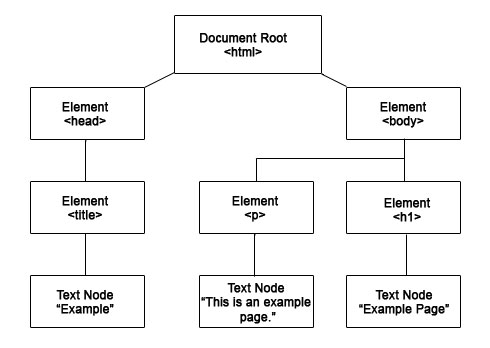
\includegraphics[width=\linewidth]{dom.jpg}
	\caption{Voorbeeld van een DOM structuur.}
	\label{fig:dom}
\end{figure}

De DOM, ofwel Document Object Model, is kortweg het skelet van een HTML-pagina. De structuur van het skelet beschrijft een boomstructuur, waardoor een element een ouder, broer, kind, kleinkind, achterkleinkind, enz... van een element kan zijn. Het HTML element is de wortel van de boom. Client-side JavaScript wordt grotendeels gebruikt om deze boomstructuur te manipuleren. Hierdoor kunnen we HTML elementen toevoegen, verwijderen, stijlen manipuleren, enz... allemaal tijdens uitvoertijd. \textcite{Kantor2017}

\subsubsection{Prototype-based}
\label{sec:prototypeBased}

In JavaScript kan een object eigenlijk aanzien worden als een Array. Hierdoor kunnen ze heel gemakkelijk aan de eigenschappen van een object aan en kunnen we deze ook makkelijk tijdens uitvoertijd aanpassen. Ook kunnen we op deze manier makkelijk eigenschappen aan bestaande objecten toevoegen. In JavaScript wordt gebruikt van de 'dot-notatie' of van de 'haakjesnotatie'. 

	\begin{verbatim}
	foo.bar = 10;
	foo['bar'] = 10;
	const bar = foo.bar;
	foo['bar2'] = bar;
	\end{verbatim}

\subsubsection{Event-driven}
\label{sec:eventDriven}

JavaScript is event-driven, wat betekent dat de code vooral kijkt naar acties van de gebruiker. Bijvoorbeeld: Wanneer een gebruiker op een knop klikt, wil je dat met een animatie de knop heeen en weer beweegt, tekst op je scherm verschijnt, en een server-request wordt gestuurd. 

\subsubsection{Functioneel}
\label{sec:functional}

Sinds ES2015 is JavaScript niet enkel en alleen een object-georiënteerde taal, maar ook een functionele taal. JavaScript was zeer snel met het introduceren van functioneel programmeren (waaronder de populaire arrow-functions). Dit vergemakkelijkte de taal aanzienlijker, aangezien veel minder code geschreven moest worden om hetzelfde resultaat te bereiken.

\subsubsection{Universeel}
\label{sec:universal}

JavaScript wordt sinds ES5 ondersteund door alle moderne browsers! Of er nu in Chrome, Firefox, Safari, Edge of het oude Internet Explorer\footnote{Internet Explorer wordt niet meer verder ontwikkelt, dus ondersteunt het enkel ES2015.} wordt gesurft, ze ondersteunen allemaal JavaScript. D.m.v. de console in de browser te openen kan er al geprogrammeerd worden.





\section{Node.js}
\label{sec:nodeJs}

Node.js is een JavaScript runtime omgeving dat wordt gebruikt voor Server-side toepassingen. Node.js maakt het mogelijk, (of eerder \textit{makkelijker}), om JavaScript nu ook te gebruiken buiten websites maken. Aangezien JavaScript zo'n krachtige taal is, hadden de ontwikkelaars van Node.js een ding in gedachten: JavaScript niet enkel in de browsers, maar ook als alleenstaande applicatie. JavaScript sindsdien evenaren aan andere scripttalen, zoals Python. \textcite{Patel2018}

\subsection{Tijdlijn van Node.js}
\label{sec:nodeTimeline}
Node.js' verhaal start in 2009, toen een ontwikkelaar genaamd Ryan Dahl het niet zo goed stelde met Apache Http Servers. 

Zoals beschreven in \autocite{Chaniotis2015}, was (en is in grote mate nog steeds) Apache HTTP, in combinatie met PHP, jarenlang de go-to-taal om webapplicaties te laten communiceren met databases en server-side functionaliteiten toe te voegen aan webapplicaties, zoals authenticatie, file-en-ftpservers, logging en nog veel meer. PHP is echter nooit in het achterhoofd ontwikkelt geweest om hedendaagse, complexe webapplicaties te schrijven. Ten tweede was Apache incapabel om te schalen naar meerdere processorkernen, waardoor de performantie enorm daalde. PHP in combinatie met Apache was gewoonweg niet gemaakt voor de volgende generatie webapplicaties. Andere struikelblokken zijn cross-platform mobiele applicaties en real-time communicatie.

Meer en meer applicaties worden gemaakt met cross-platform compatibiliteit in het achterhoofd, aangezien de toestroming van verschillende nieuwe besturingssystemen en apparaten het meer en meer onmogelijk maken om native apps\footnote{Native Apps zijn applicaties die gemaakt worden met één besturingssysteem in het hoofd. Bv: Android, IOS.} te ontwikkelen. Hierdoor worden bibliotheken en frameworks ontwikkelt zoals React Native, Flutter, Xamarin, Ionic, PhoneGap, enz... die deze nadelen kunnen overbruggen. Deze zijn echter zo krachtig geworden en schenken zoveel nieuwe voordelen, dat server-side talen en frameworks zoals Apache HTTP/PHP eerder een bottleneck vormden. 

Real-time communicatie is nog een factor dat niet ondersteunt wordt door Apache. Apache was niet ontwikkelt om berichten te sturen naar de client-side. In de wereld van vandaag, waarin sociale media nog nooit zo'n grote invloed heeft gehad op ons dagelijks leven, is het haast ondenkbaar dat real-time communicatie niet zou kunnen bestaan. 

Dit alles zorgde voor de ontwikkeling van Node.js. Dahl's project werd met open armen ontvangen. Na enkele struikelblokken, kende Node.js in 2011 voor het eerst het licht en wordt nu zo'n tien jaar later, gebruikt in vele moderne applicaties en is nog steeds één van de meest begeerde vaardigheden van een programmeur. \autocite{Patel2018}

Hoewel Apache en PHP nog steeds overduidelijk op plaats één staan, hebben ze hun populariteit enkel nog te danken aan bedrijven die op verouderde software werken, en hun populariteit bij senior ontwikkelaars. PHP blijft een geliefde taal bij velen, maar we zien dat Node.js populariteit duidelijk die van Apache aan het inhalen is. \autocite{SimilarTech}

\begin{figure}[h]
	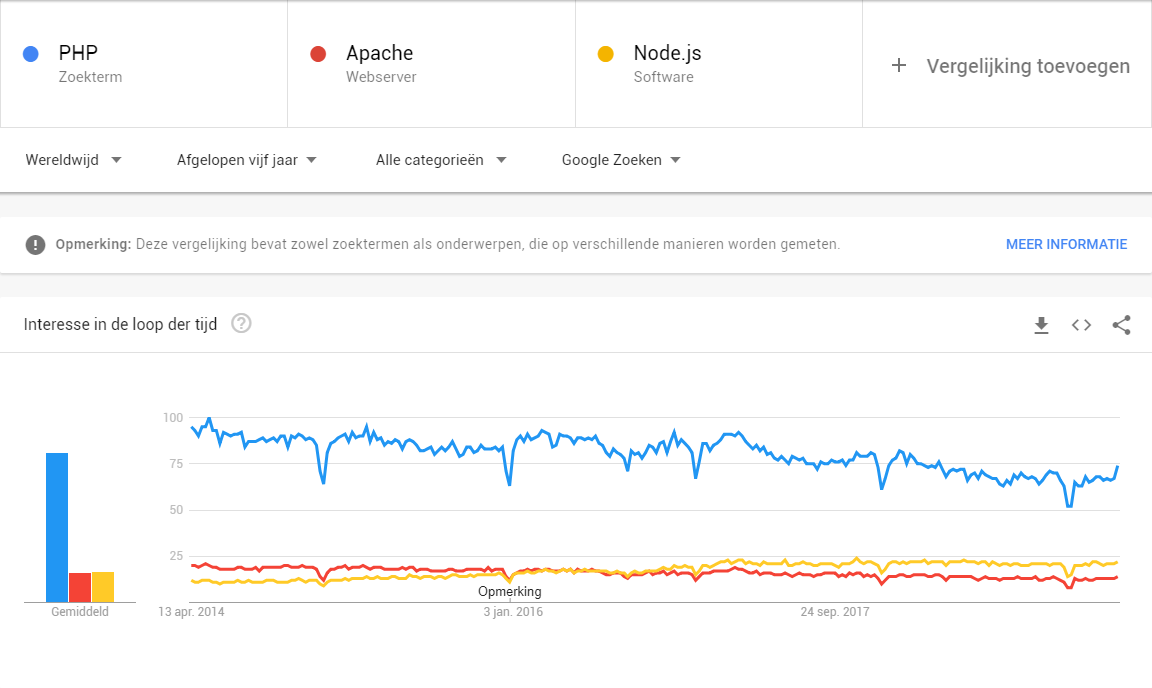
\includegraphics[width=\linewidth]{trend.png}
	\caption{Google searches van PHP (blauw), Apache (rood) en Node.js (geel) in de afgelopen 5 jaar.}
	\label{fig:trend}
\end{figure}

\subsection{Waarom Node.js?}
\label{sec:whyNode}
Node.js is reeds een volwassen server-side framework. Youtube, Yahoo, Google, Amazon, Netflix, Ebay, Reddit, LinkedIn, Paypal, Github, Forbes, Walmart, Uber, NASA, Slack,.. zijn slechts enkele van de duizenden websites die overgeschakeld zijn naar Node.js. En dit zijn geen kleine namen.

Illustrator \textcite{Mehmet2016} toont op een illustratieve wijze de voordelen van Node.js aan. LinkedIn kon hun 15 servers reduceren naar slechts 4 en terwijl de verkeerscapaciteit nog eens verdubbelen. Walmart kon al hun Client-side JavaScript processing naar hun servers verplaatsen, en Ebay kon hun verkeerscapaciteit enorm doen verhogen en hun verbruik enorm doen dalen. De voordelen en functionaliteiten worden hieronder nog eens opgesomd zoals aangegeven door \textcite{Chandrayan2017}.

\subsubsection{Asynchroon}
\label{sec:async}

Node.js is sterk afhankelijk van asynchrone en continue programmeerstijl. I/O-bewerkingen worden uitgevoerd door middel van oproepen naar asynchrone functies waarbij een callback moet worden doorgegeven om aan te geven hoe de berekening wordt voortgezet zodra de genoemde I/O-bewerking asynchroon is voltooid. Het Node.js executiemodel bestaat uit een hoofdgebeurtenislus die wordt uitgevoerd op een single-threaded proces. dankzij deze \textit{event loop} moet een Node.js server nooit wachten op antwoord, het kan gewoon blijven doordraaien na een oproep van een API Call en kan dankzij een notificatiesysteem op een later moment het antwoord terugsturen. Dit maakt Node.js enorm schaalbaar, in tegenstelling tot Apache dat slechts een gelimiteerd aantal threads kan starten om handelingen uit te voeren.

Het is daarom niet altijd makkelijk om deze soort frameworks te debuggen, en het wordt uiteindelijk een uitdagende taak. Gelukkig zijn hiervoor dan ook weer verschillende hulpmiddelen en tools uitgebracht om dit te vereenvoudigen. Zoals hierboven vermeld in ~\autocite{Runtime2017}, kan asynchrone code subtiele bugs opleveren die niet meteen zichtbaar zijn.  Hier is nog niet echt onderzoek over gedaan. Waarin er honderden vergelijkende studies bestaan over de frameworks zelf en of Node.js een goede optie is, zijn er geen of amper studies over de beste manier om dit te debuggen en hoe men dit het best aanpakt. ~\autocite{Runtime2017} vertelt ons meer over het identificeren van schaalbaarheidsproblemen en het aanrijken van mogelijke oplossingen. Ze maken gebruik van parametrische uitdrukkingen voor runtime monitoring van Node.js toepassingen, maar ze geven toe dat dit nog maar de eerste stap is en dat hier nog meer onderzoek naar kan gedaan worden. Hier wordt later in dit onderzoek dieper op ingegaan.

\subsubsection{Performant}
\label{sec:fast}

Google Chrome's JavaScript engine, V8, is bijzonder snel. Dahl heeft dit verder ontwikkeld voor Node.js en dit maakt de framework enorm performant en efficiënt in het uitvoeren van code. Veel sneller dan Python, Ruby of Perl.

\subsubsection{NPM}
\label{sec:npm}

Node.js kent een enorm bloeiende community. Deel van Node is zijn Node Package Manager, ofwel npm, en komt meegeleverd bij de installatie. Via npm kan men uit honderdduizenden pakketjes kiezen voor een JavaScript/Node project makkelijk uit te breiden met extra functionaliteiten in één oogwenk. Dagelijks worden er nieuwe pakketjes toegevoegd aan de packet manager, en is makkelijk één van de redenen waarom Node.js zo populair is, aangezien het ontwikkelen van een webapplicatie enorm vereenvoudigd wordt.   



\section{Express}
\label{sec:express}




 






 
